Note que en este caso parece apropiada utilizar un cambio de variable con coordenadas esféricas, pues $W$ esta acotada por esferas y sabemos que $x^2 + y^2 + z^2$ puede remplazarse por $p^2$, obteniendo así una integral mucho más sencilla. Además, la región descrita en este ejercicio es la que se encuentra entre las dos esferas siguientes, donde la interior tiene un radio $b$ y la exterior un radio $a$

\begin{center}
	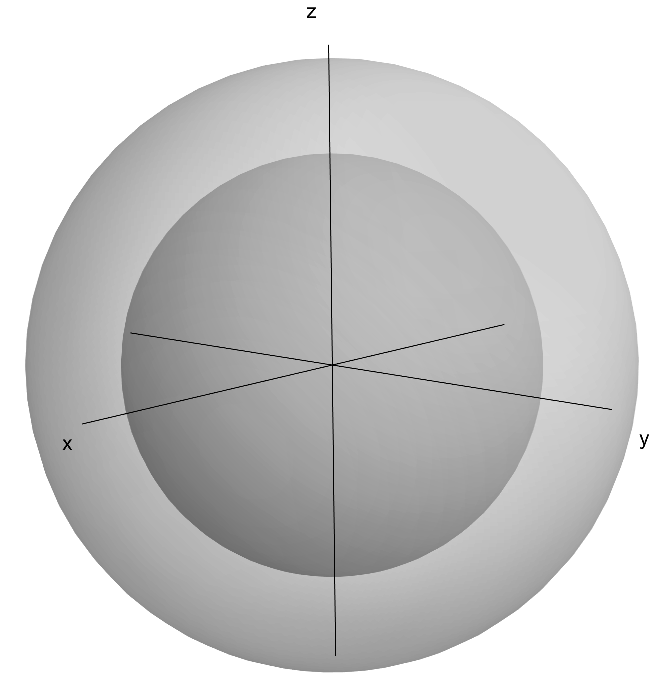
\includegraphics[width=0.35\linewidth]{figuras/esferas-ej25.pdf}
\end{center}

Entonces, si $W^*$ es la región dada por
\[b \leq p \leq a, \qquad 0 \leq \theta \leq 2\pi, \qquad 0 \leq \phi \leq \pi\]

Aplicando la fórmula del cambio de variables con coordenadas esféricas

\[\iiint_W \frac{dx\, dy\, dz}{(x^2 + y^2 + z^2)^{3/2}}	= \iiint_{W^*} \frac{1}{(p^2)^{3/2}} \cdot p^2\sen\phi\, dp\, d\theta\, d\phi = \iiint_{W^*} \frac{1}{p} \sen \phi\, dp\, d\theta\, d\phi\]

Y por el terorema de Fubini esta última integral es igual a la siguiente integral iterada
\begin{align*}
	\int_{0}^{2\pi} \int_{0}^{\pi} \int_b^a\frac{1}{p} \sen\phi \, dp\, d\phi\, d\theta &= \int_{0}^{2\pi} \int_{0}^{\pi} \left[\ln|p| \sen\phi\right]_{p=b}^{p=a} \, d\phi\, d\theta\\
	&= \int_{0}^{2\pi} \int_{0}^{\pi} \ln\left(\frac{a}{b}\right) \sen\phi \, d\phi\, d\theta\\
	&= \ln\left(\frac{a}{b}\right) \int_{0}^{2\pi} \int_{0}^{\pi} \sen\phi \, d\phi\, d\theta\\
	&= \ln\left(\frac{a}{b}\right) \int_{0}^{2\pi} [-\cos\phi]_{\phi=0}^{\phi=\pi}\, d\theta\\
	&= \ln\left(\frac{a}{b}\right) \int_{0}^{2\pi} 2\, d\theta\\
	&= 2\ln\left(\frac{a}{b}\right) \int_{0}^{2\pi} d\theta\\
	&= 2\ln\left(\frac{a}{b}\right) (2\pi)\\
	&= 4\pi\ln\left(\frac{a}{b}\right)
\end{align*}

Por lo tanto
\[\iiint_W \frac{dx\, dy\, dz}{(x^2 + y^2 + z^2)^{3/2}} = 4\pi\ln\left(\frac{a}{b}\right)\]